\documentclass[a4paper,11pt]{article}
%
% document setup, package import, etc.
%
%
% packages and settings for the worksheet files
%
\usepackage[bf,small]{titlesec}
\usepackage{graphicx}
\usepackage{amsfonts,amssymb,amsmath,fancyhdr}
%\usepackage{import} % needed for subimport
\usepackage{url}
\usepackage{paralist} % needed for compactenum
\usepackage{verbatim} % needed for varbatimiinput
\usepackage{shortlst}
\usepackage{siunitx}
%
%  page layout
%
\setlength{\textwidth}{175mm}
\setlength{\textheight}{240mm}
\setlength{\voffset}{-20mm}
\setlength{\hoffset}{-23mm}
\setlength{\parskip}{0pt}
\setlength{\parindent}{0pt}
\setlength{\footskip}{40pt}
\renewcommand{\baselinestretch}{1.2} \small\normalsize
%
%  Header/footer
%
\fancyhf{} % Clear all fields
\renewcommand{\headrulewidth}{0pt}
\renewcommand{\footrulewidth}{0pt}
\fancyfoot[L]{\footnotesize EMAT20920 2020-21}
\fancyfoot[C]{\footnotesize \thepage}
\fancyfoot[R]{\footnotesize Coursework Assessment}
%
% Change list-making
%
\renewcommand{\theenumi}{\alph{enumi}}
\def\labelenumi{(\theenumi)}
\renewcommand{\theenumii}{\roman{enumii}}
\def\labelenumii{(\theenumii)}
%
% Change section headers
%
\titlelabel{Question \thetitle:\quad}
%
% First page header
%
\newcommand{\solutionsheader}[2]{
    \pagestyle{fancy}
    \begin{center}
      {\large Department of Engineering Mathematics}\\[3ex]
      \textbf{EMAT20920: Numerical Methods in MATLAB}\\[3ex]
      \textbf{#1}\\
      \textbf{#2}
    \end{center}}
%
% For formatting matlab code with listings
%
\usepackage{listings}
\usepackage{color}
\usepackage{textcomp}
\definecolor{listinggray}{gray}{0.9}
\definecolor{lbcolor}{rgb}{0.9,0.9,0.9}
\lstset{
    backgroundcolor=\color{lbcolor},
    numbers=none,
    numberstyle=\tiny,
    tabsize=4,
    rulecolor=,
    language=matlab,
    basicstyle=\scriptsize\ttfamily,
    upquote=true,
    aboveskip={1.5\baselineskip},
    columns=flexible,
    showstringspaces=false,
    extendedchars=true,
    breaklines=true,
    prebreak = \raisebox{0ex}[0ex][0ex]{\ensuremath{\hookleftarrow}},
    %frame=single,
    showtabs=false,
    showspaces=false,
    showstringspaces=false,
    identifierstyle=\ttfamily,
    keywordstyle=\color[rgb]{0,0,1},
    commentstyle=\color[rgb]{0.133,0.545,0.133},
    stringstyle=\color[rgb]{0.627,0.126,0.941},
    aboveskip=0pt,
    belowskip=2pt,
}

%%%

\newcommand\NoIndent[1]{%
	\par\vbox{\parbox[t]{\linewidth}{#1}}%
}
%
% shortcut commands
%
\newcommand{\matcmd}[1]{\colorbox{lbcolor}{\lstinline{#1}}}
\newcommand{\matlab}[1]{\texttt{#1}}
\renewcommand{\vec}[1]{\boldsymbol{#1}}
\newcommand{\order}{\mathcal{O}}

\newenvironment{listcomment}[1][1]{\framed\adjustwidth{-\dimexpr 
#1\leftmargin + \fontdimen2\font}{}}{\endadjustwidth\endframed}

\usepackage[toc,title]{appendix}
\usepackage{caption}
\usepackage[backend=bibtex8]{biblatex}
\addbibresource{ref.bib}

\usepackage{hyperref}

\begin{document}

\solutionsheader{COURSEWORK ASSESSMENT}{Jake Bowhay (UP19056)}

\tableofcontents

\hfill \break

All figures in this report have been saved using \verb*|saveFigPDF| function 
as it automatically resizes the paper to the correct size.
\lstinputlisting{../src/saveFigPDF.m}

\section{Root-finding}
\begin{enumerate}
	\item To find how many solutions each equation has in the domain  I 
	will rearrange all the equations to be equal to zero and then looks for 
	the roots of the rearranged equations. As a corollary to the intermediate 
	value theorem, if a function is continuous and changes sign in an 
	interval 
	then that bracketing interval must contain a root. So I will plot each of 
	the 
	rearranged equation and look for bracketing intervals that contain a 
	root. I will use the 
	\verb*|pltFunc| function (as shown in \autoref{lst:pltFunc}) to plot the 
	functions as it removes values 
	outside a defined limit which prevents MATLAB plotting discontinuous 
	functions as continuous. The limits can then be changed using the 
	property explorer to show more detail if needed.
	\begin{enumerate}
		\item Rearranging $x^{4} = e^{-x} \cos(x)$ gives $f(x) = x^{4} - 
		e^{-x} \cos(x)$.
		\lstinputlisting{../src/q1/Q1a_i_funcPlt.m}
		\NoIndent{
			\includegraphics[scale=0.5]{images/Q1a_i.pdf}
			\includegraphics[scale=0.5]{images/Q1a_i_zoomed.pdf}
		}
			The second zoomed plot shows there are two solutions in the 
			given domain.
			\begin{center}
				\begin{tabular}{l|lll}
					$[a,b]$     & f(a)    & f(b)    & Continuous over $[a,b]$ 
					\\ \hline
					$[-1.5,-1]$ & 4.7455  & -0.4687 & Yes                     
					\\
					$[0.5,1]$   & -0.4698 & 0.8012  & Yes                    
				\end{tabular}
			\end{center}
			
			
		\item Setting $f(x) = \frac{x^{3}}{\sin(x)} - 1$.
			\lstinputlisting{../src/q1/Q1a_ii_funcPlt.m}
		\NoIndent{
			\includegraphics[scale=0.5]{images/Q1a_ii.pdf}
			\includegraphics[scale=0.5]{images/Q1a_ii_zoomed.pdf}
		}
		The second plot shows there are two roots. 
		\begin{center}
			\begin{tabular}{l|lll}
				$[a,b]$     & f(a)    & f(b)    & Continuous over $[a,b]$ \\ 
				\hline
				$[-1,-0.5]$ & 0.1884  & -0.7393 & Yes                     \\
				$[0.5,1]$   & -0.7393 & 0.1884  & Yes                    
				\end{tabular}
		\end{center}
		
		
		\item Rearranging $\cot(x) = \frac{25}{25x-1}$ gives $f(x) = \cot(x) 
		- \frac{25}{25x-1}$.
		\lstinputlisting{../src/q1/Q1a_iii_funcPlt.m}
		\begin{center}
			\includegraphics[scale=0.5]{images/Q1a_iii.pdf}
		\end{center}
		The plot shows that the equation has three solutions. 
		\begin{center}
			\begin{tabular}{l|lll}
				$[a,b]$     & f(a)   & f(b)    & Continuous over $[a,b]$ \\ 
				\hline
				$[-5,-4]$   & 0.4942 & -0.6162 & Yes                     \\
				$[-1,-0.1]$ & 0.3194 & -2.8238 & Yes                     \\
				$[4,5]$     & 0.6112 & -0.4974 & Yes                    
			\end{tabular}
		\end{center}
	
	
		\item Rearranging $4e^{-x^{2}/5} = cos(5x) + 2$ gives $f(x) = 
		4e^{-x^{2}/5} - cos(5x) - 2$.
		\lstinputlisting{../src/q1/Q1a_iv_funcPlt.m}
		\NoIndent{
		\includegraphics[scale=0.5]{images/Q1a_iv.pdf}
		\includegraphics[scale=0.5]{images/Q1a_iv_zoomed.pdf}
		}
		The second plot shows that the equation has 6 solutions. The 
		bracketing intervals are shown in the table below.
		\begin{center}
			\begin{tabular}{l|lll}
				$[a,b]$        & f(a)    & f(b)    & Continuous over $[a,b]$ 
				\\ \hline
				$[-2.5,-2]$    & -1.8518 & 0.6364  & Yes                     
				\\
				$[-1.5,-1.25]$ & 0.2039  & -0.0730 & Yes                     
				\\
				$[-1.25,-1]$   & -0.0730 & 0.9913  & Yes                     
				\\
				$[1,1.25]$     & 0.9913  & -0.0730 & Yes                     
				\\
				$[1.25,1.5]$   & -0.0730 & 0.2039  & Yes                     
				\\
				$[2,2.5]$      & 0.6364  & -1.8518 & Yes                    
			\end{tabular}
		\end{center}
	\end{enumerate}



	\item The bisection method is used by calling the \verb*|bisectRoot| 
	function.
	\lstinputlisting[label=lst:bisect]{../src/q1/bisectRoot.m}
	
	
	\begin{enumerate}
		\item Solutions to $f(x) = x^{4} - e^{-x} \cos(x) = 0 \  \ 
		x\in[-2\pi,2\pi]$.
		\lstinputlisting{../src/q1/Q1b_i_funcRoots.m}
		Note the two different tolerances since one root is an order of 
		magnitude larger so requires one less decimal place of tolerance to 
		be 
		accurate to 8 significant figures.
		\begin{center}
			\begin{tabular}{l|ll}
				$[a,b]$     & Root       & \# Iterations \\ \hline
				$[-1.5,-1]$ & -1.084359675645828 & 23           \\
				$[0.5,1]$   & 0.762211065739393 & 26          
			\end{tabular}
		\end{center}
		
	
	
		\item Solutions to $f(x) = \frac{x^{3}}{\sin(x)} - 1 = 0 \  \ 
		x\in[-2\pi,2\pi]$.
		\lstinputlisting{../src/q1/Q1b_ii_funcRoots.m}
		\begin{center}
			\begin{tabular}{l|ll}
				$[a,b]$     & Root        & \# Iterations \\ \hline
				$[-1,-0.5]$ & -0.928626310080290 & 26            \\
				$[0.5,1]$   & 0.928626310080290  & 26           
			\end{tabular}
		\end{center}
	
	
		\item Solutions to $f(x) = \cot(x)	- \frac{25}{25x-1} = 0 \  \ 
		x\in[-2\pi,2\pi]$.
		\lstinputlisting{../src/q1/Q1b_iii_funcRoots.m}
		Again note the different tolerances due to the different orders of 
		magnitude of the roots.
		\begin{center}
			\begin{tabular}{l|ll}
				$[a,b]$     & Root        & \# Iterations \\ \hline
				$[-5,-4]$   & -4.495372205972672  & 24            \\
				$[-1,-0.1]$ & -0.477733755484223 & 27            \\
				$[4,5]$     & 4.491409689188004   & 24           
			\end{tabular}
		\end{center}
		
		
		\item Solutions to $f(x) = 4e^{-x^{2}/5} - cos(5x) - 2 = 0 \  \ 
		x\in[-2\pi,2\pi]$.
		\lstinputlisting{../src/q1/Q1b_iv_funcRoots.m}
		\begin{center}
			\begin{tabular}{l|ll}
				$[a,b]$        & Root       & \# Iterations \\ \hline
				$[-2.5,-2]$    & -2.122238188982010 & 23            \\
				$[-1.5,-1.25]$ & -1.425543159246445 & 22            \\
				$[-1.25,-1]$   & -1.214593321084976 & 22            \\
				$[1,1.25]$     & 1.214593321084976  & 22            \\
				$[1.25,1.5]$   & 1.425543159246445  & 22            \\
				$[2,2.5]$      & 2.122238188982010  & 23           
			\end{tabular}
		\end{center}
	\end{enumerate}


	\item The iterative scheme we asked to implement is called Steffensen's 
	method\cite{wiki:Steffensen's_method}. This is implemented in the 
	\verb*|steffensenRoot| function.
	\lstinputlisting[label=lst:steph]{../src/q1/steffensenRoot.m}
	The following uses this function to find the root of $e^{-x} - x = 0$ and 
	calculate the convergence.
	\lstinputlisting{../src/q1/Q1c_errorConvergance.m}
	After 5 iterations the root $x = 0.567143290409784$ is accurate to 12 
	decimal places.
	\begin{center}
		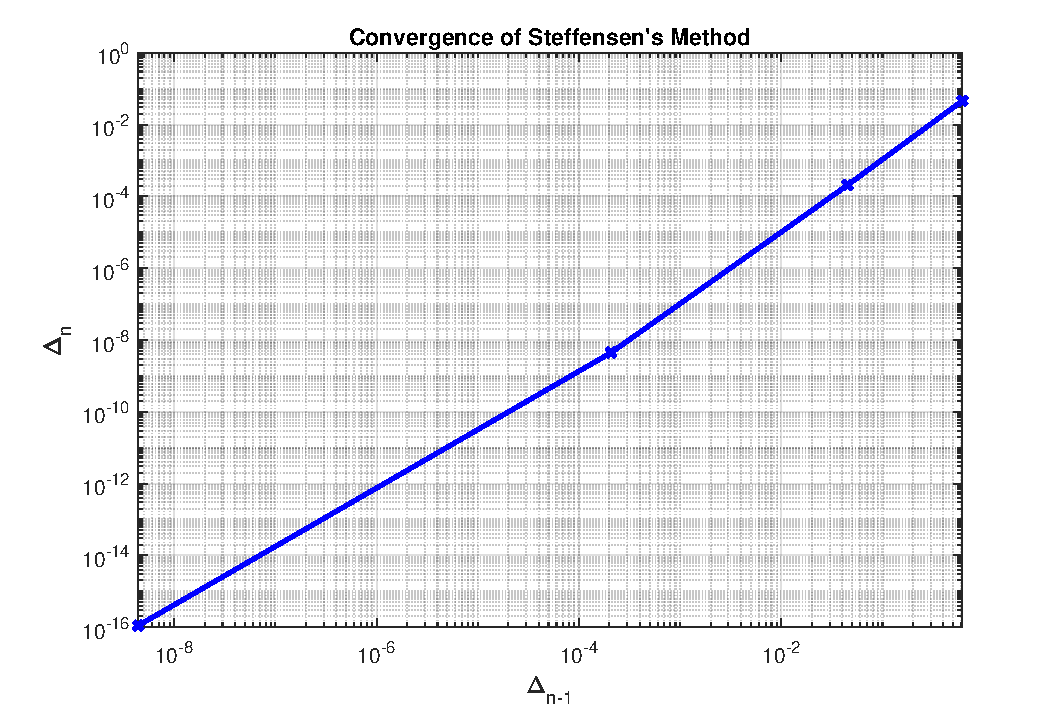
\includegraphics[scale=0.6]{images/Q1c.pdf}
	\end{center}
	The graph shows a straight which shows error $\propto \Delta_{n-1}^{q}$, 
	where q is the gradient of the line. Using the \verb*|MATLAB| function 
	\verb*|polyfit| the gradient of the 
	above graph as 1.8. The absolute error is an approximate so this can be 
	approximated to 2 meaning Steffensen's method is second order.
	
	
	\item The first step in creating a cobweb plot is to implement a fixed 
	point iteration scheme.
	\lstinputlisting{../src/q1/fixedPointRoot.m}
	Then the \verb*|cobwebDiagram| function can display the results of the 
	fixed point iteration.
	\lstinputlisting{../src/q1/cobwebDiagram.m}
	The function requires user inputs of the iteration function $g(x)$, 
	the initial guess $x_{0}$, the number of iterations and the interval to 
	display on the x-axis (which should contain the root). The reason to user 
	has to enter the range to display on the x-axis is because in the case of 
	divergence the estimate of the root can shoot off to very large value 
	which when plotted make previous iteration so small that the plot doesn't 
	show anything meaningful.
	
	The first test I did was to ensure it could produce a cobweb diagram. For 
	this I set $g(x) = \frac{3 - x^{3}}{4}$ with an initial guess of 
	$\frac{1}{2}$.
	\lstinputlisting{../src/q1/Q1d_cobweb_example.m}
	\begin{center}
		\includegraphics[scale=0.6]{images/Q1d_cobweb.pdf}
	\end{center}

	Next I tested producing a staircase diagram, so I set $g(x) = 
	\sqrt[5]{5x-3}$ with an initial guess of 1.
	\lstinputlisting{../src/q1/Q1d_staircase_example.m}
	\begin{center}
		\includegraphics[scale=0.6]{images/Q1d_staircase.pdf}
	\end{center}
	Since the function should also be able to handle iterations that don't 
	converge, I tried $g(x)=\frac{1-xe^{x}}{x}$ with an initial guess of 
	$\frac{1}{2}$.
	\lstinputlisting{../src/q1/Q1d_divergance_example.m}
	\begin{center}
		\includegraphics[scale=0.6]{images/Q1d_divergance.pdf}
	\end{center}
	This cobweb diagram shows how the gradient at the root is too steep which 
	means the iteration fails to converge. This is also shown by that fact 
	that the approximate absolute error at the final step is still $\sim4.6$. 
	I also tested it with a number of other function both converge and 
	diverge however these have been omited from the report to save space.
\end{enumerate}

\section{Numerical integration and differentiation}
\begin{enumerate}
	\item \begin{enumerate}
		\item The first of the given expression is Simpson's 3/8 rule and the 
		second given expression is 
		Milne's rule\cite{wiki:nc}.
		
		Simpson's 3/8 rule can be implemented as follows.
		\lstinputlisting{../src/q2/simpson38.m}
		And similarly Milne's rule can be implemented.
		\lstinputlisting{../src/q2/milne.m}
		However, to use the composite version the integral must be broken 
		down 
		into smaller intervals. For example breaking the integral into $n$ 
		intervals gives $\int_{a}^{b}f(x)dx = \int_{a}^{x_{1}}f(x)dx + 
		\int_{x_{1}}^{x_{2}}f(x)dx + \cdots + \int_{x_{n-1}}^{b}f(x)dx$ 
		where 
		$x_{i} = a + i \cdot \frac{b - a}{n}$. Then each of these smaller 
		integrals can be calculated using either of the methods. The 
		\verb*|compositeQuad| function breaks down the integral into smaller 
		intervals before using a Newton-Coutes method of choice to 
		approximate the integral.
		\lstinputlisting{../src/q2/compositeQuad.m}
		For an example both methods can be used to evaluate $\int_{0}^{5} 
		e^{x} - x dx$ to 6 decimal places as follows.
		\lstinputlisting{../src/q2/Q2ai_exampleIntegration.m}
		Both give the answer to the example as $134.913159$.
		
		
		\item The order of a Newton-Cotes method is measured with respect to 
		$h$ (the size of subintervals).
		\begin{center}
			\includegraphics[scale=0.7]{images/Q2aii.pdf}
			\captionof{figure}{Error convergance of composite Simpson's 3/8 
			rule and composite
			Milne's rule. 
			Generated using 
			\autoref{lst:q2aii}.}
			\label{fg:interr}
		\end{center}
		\autoref{fg:interr} shows both method produce a straight line which 
		shows error $\propto h^{q}$ where q is the gradient. The 
		\verb*|polyfits| function shows both line have a gradient of 4 which 
		means both composite Simpson's 3/8 rule and composite Milne's rule 
		are 4th order.
		
		The accuracy is the highest order polynomial that the method can 
		integrate exactly. So to find the degree of accuracy of each method 
		test it on a variety of polynomials of increasing order and see if it 
		can integrate the polynomial exactly.
		
		\begin{center}
			\begin{tabular}{l|lll}
				& Exact Value    & Simpon's 3/8 Rule & Milne's Rule      \\ 
				\hline
				$\int_{0}^{1}x \ dx$     & $\frac{1}{2}$ & 0.5               
				& 0.5               \\
				$\int_{0}^{1}x^{2} \ dx$ & $\frac{1}{3}$ & 0.333333333333333 
				& 0.333333333333333 \\
				$\int_{0}^{1}x^{3} \ dx$ & $\frac{1}{4}$ & 0.25              
				& 0.25              \\
				$\int_{0}^{1}x^{4} \ dx$ & $\frac{1}{5}$ & 0.203703703703704 
				& 0.192708333333333
			\end{tabular}
		\end{center}
		This shows that both methods are of degree of accuracy 3 as they can 
		both exact integrate cubics but not quartics.
		
		Whilst both methods are fourth order Simpson's 3/8 rule has a lower 
		error term so is slightly better as it is more accurate. This is 
		shown in \autoref{fg:interr} as the absolute error for Simpson's 
		3/8 rule is always less.
	\end{enumerate}

	
	\item \begin{enumerate}
		\item To find the order of the rounding and truncation error when 
		numerically approximating $f''(x)$ the absolute error is plotted 
		against $h$. Since $f(x)$ given is differentiable 
		$f''(x)$ can be found exactly and then the absolute error can be 
		found by subtracting \autoref{eq:f''} from the numerical 
		approximation. The exact second derivative is
		\begin{equation}
			\frac{d^{2}}{dx^{2}}(\sin^{3}(x)) = -3\sin^{3}(x) + 
			3\cos(x)\sin(2x).
			\label{eq:f''}
		\end{equation}
		\begin{center}
			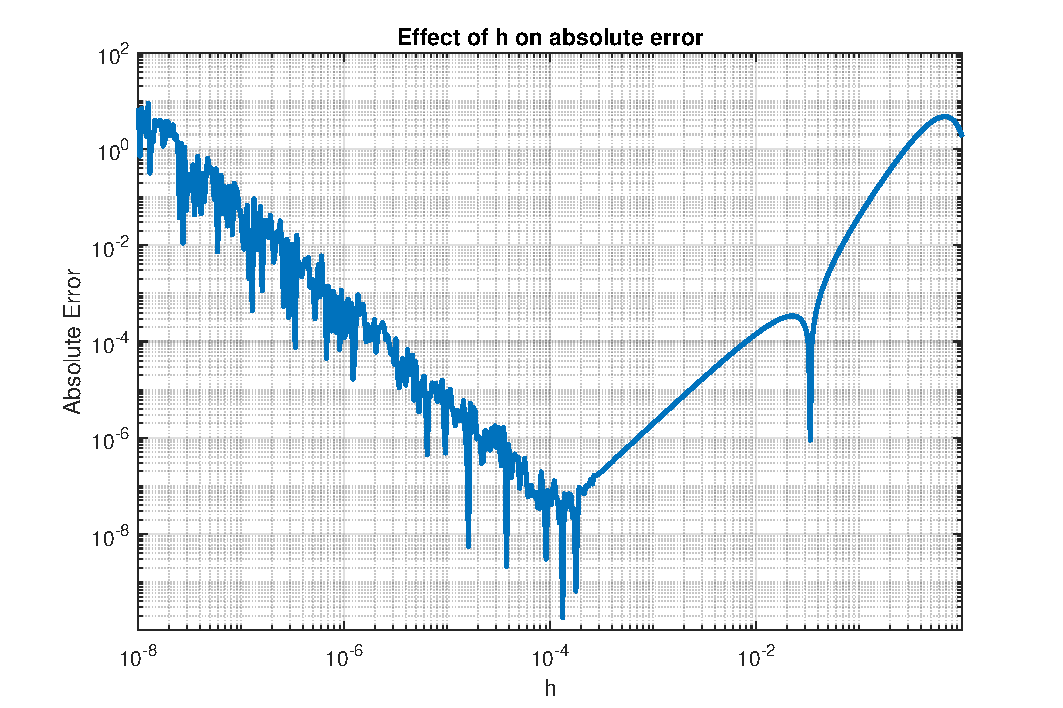
\includegraphics[scale=0.7]{images/Q2bi.pdf}
			\captionof{figure}{Plot generated by \autoref{lst:q2bi}}
		\end{center}
		The gradient of the two sections of the graph shows the order of the 
		rounding and truncation error. The rounding error is shown by the 
		jagged first half which has a gradient of -2 which shows the order of 
		the rounding error is $\mathcal{O}(h^{-2})$. The second half of the 
		graph shows the truncation error. This has a gradient of 2 which 
		shows the truncation error is $\mathcal{O}(h^{2})$.
		
		\item The error comprises the truncation and rounding error. To 
		find the truncation error of 
		\begin{equation}
			f''(x) \approx \frac{2f(x)-5f(x+h)+4f(x+2h)-f(x+3h)}{h^{2}},
			\label{eq:f''}
		\end{equation}
		consider the following Taylor expansions
		\begin{equation}
			f(x + h) = f(x) + hf'(x) + \frac{h^{2}}{2}f''(x) + 
			\frac{h^{3}}{6}f^{(3)}(x) + \frac{h^{4}}{24}f^{(4)}(x) + \cdots,
			\label{eq:t1}
		\end{equation}
		\begin{equation}
			f(x + 2h) = f(x) + 2hf'(x) + \frac{4h^{2}}{2}f''(x) + 
			\frac{8h^{3}}{6}f^{(3)}(x) + \frac{16h^{4}}{24}f^{(4)}(x) + 
			\cdots,
			\label{eq:t2}
		\end{equation}
		\begin{equation}
			f(x + 3h) = f(x) + 3hf'(x) + \frac{9h^{2}}{2}f''(x) + 
			\frac{27h^{3}}{6}f^{(3)}(x) + \frac{81h^{4}}{24}f^{(4)}(x) + 
			\cdots.
			\label{eq:t3}
		\end{equation}
		Substituting \eqref{eq:t1}, \eqref{eq:t2}, \eqref{eq:t3} into 
		\eqref{eq:f''} gives
		\begin{align}
			f''(x) &\approx \frac{h^{2}f''(x) + 
			\frac{-11}{12}h^{4}f^{(4)}(x) + \mathcal{O}(h^{5})}{h^{2}}\\
			&= f''(x) - \frac{11}{12}h^{2}f^{(4)}(x) + 
			\mathcal{O}(h^{3}),
		\end{align}
		so the truncation error is $\frac{11}{12}h^{2}f^{(4)}(x) + 
		\mathcal{O}(h^{3})$.
		
		To find the rounding error assume $h$ is small and can be stored 
		exactly. So the rounding error in storing $f(x)$, $f(x+h)$, $f(x+2h)$ 
		and $f(x+3h)$ is $|f(x)|\epsilon$, where $\epsilon$ is the floating 
		point relative accuracy, $2\times 10^{-16}$. This means the total 
		rounding error is $\frac{12|f(x)|\epsilon}{h^{2}}$. So the total 
		error is given by
		\begin{equation}
			\text{error} \approx \frac{11}{12}h^{2}f^{(4)}(x) + 
			\frac{12|f(x)|\epsilon}{h^{2}}.
		\end{equation}
		We want to minimise the error so
		\begin{equation}
			\frac{d}{dt}\text{error} \approx \frac{22}{12}hf^{(4)}(x) - 
			\frac{24|f(x)|\epsilon}{h^{3}}=0.
		\end{equation}
		Approximating $f(x)\approx f^{(4)}(x)$ gives
		\begin{equation}
			\frac{22}{12}h - 
			\frac{24\epsilon}{h^{3}}=0,
		\end{equation}
		so the h which minimises the error is
		\begin{equation}
			h = \sqrt[4]{\frac{144}{11}\epsilon}.
		\end{equation}
		\begin{center}
			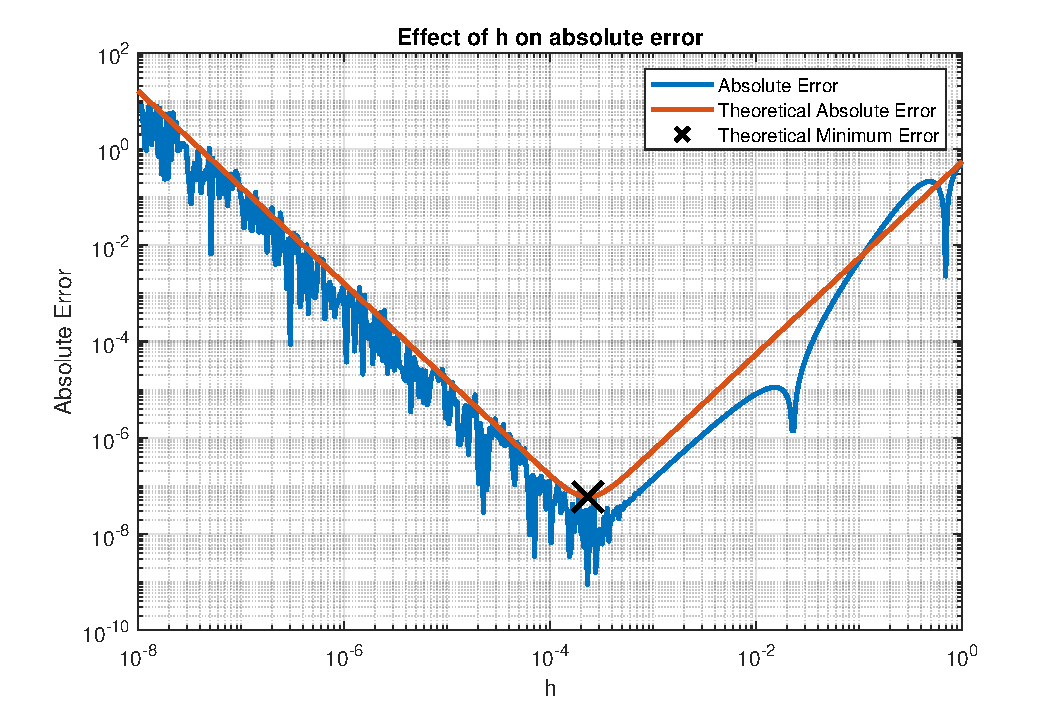
\includegraphics[scale=0.7]{images/Q2bii.pdf}
			\captionof{figure}{Plot produced using \autoref{lst:q2bii}}
		\end{center}
		The algebraic expression has the same gradient however it is offset. 
		This is because it assumes that $h$ can be stored exactly and because 
		it assumes $f(x)\approx f^{(4)}(x)$. However, the value of h that 
		minimises error lines up correctly.
	\end{enumerate}
\end{enumerate}

\section{Numerical solution of ODEs}
\begin{enumerate}
	\item \lstinputlisting{../src/q3/rhsProjectile.m}
	
	
	\item\begin{enumerate}
		\item Forward Euler
		\lstinputlisting{../src/q3/forwardEulerProjectile.m}
		\item 4th-order Runge-Kutta
		\lstinputlisting{../src/q3/rk4Projectile.m}
		\item \verb*|ode45|
		\lstinputlisting{../src/q3/ode45projectile.m}
	\end{enumerate}


	\item Solving the ODE using the three solvers gives the 
	following different trajectories.
	\begin{center}
		\includegraphics[scale=0.7]{images/Q3c.pdf}
		\captionof{figure}{Comparision of the three different solutions. Plot 
		produced using \autoref{lst:q3c}}
	\end{center}

	
	\item Global truncation error of forward Euler compared to \verb*|ode45|.
	\begin{center}
		\includegraphics[scale=0.7]{images/Q3d.pdf}
		\captionof{figure}{Generated using \autoref{lst:q3d}}
	\end{center}
	The order of global truncation error can be given by the gradient in the 
	limit as $h \xrightarrow{} 0$. In this case the gradient is 1 so the 
	global truncation error is $\order(h)$.
	
	\item To find when the projectile crosses the x-axis first an event 
	function is created.
	\lstinputlisting{../src/q3/xaxisEvent.m}
	Then solve the ODE with the added event function.
	\lstinputlisting{../src/q3/Q3e_eventDetection.m}
	This gives that the projectile first passes through the x-axis when 
	$t=3.038777368718$
	
	
	\item An equivalent formulation to this problem is to consider the angles 
	$\theta_{0}$ required so that when a particle is fired from $(-40,0)$ it 
	lands through the origin $(0,0)$. This can be visualized by plotting the 
	landing $x$ coordinate against $\theta_{0}$ as shown in 
	\autoref{fg:landing}.
	\begin{center}
		\includegraphics[scale=0.7]{images/Q3f.pdf}
		\captionof{figure}{Generated using \autoref{lst:q3f}}
		\label{fg:landing}
	\end{center}
	This shows the problem can be reduced to a root finding problem. This can 
	be done using the bisection method already implemented in 
	\autoref{lst:bisect} or Stephen's method implemented in 
	\autoref{lst:steph}. The two values of $\theta_{0}$ can be bracketed by 
	the 
	intervals $[20,25]$ and $[50,55]$. First a function, $x(\theta_{0})$, 
	that 
	returns just the 
	landing 
	position given a $\theta_{0}$ needs to be created.
	\lstinputlisting{../src/q3/landingPosition.m}
	Then using the bisection method the roots of $x(\theta_{0}) = 0$ can be 
	found.
	\lstinputlisting{../src/q3/Q3f_thetaSolution.m}
	This gives $\theta_{0} = 21.9185709$ or $\theta_{0} = 51.567361$ as 
	solutions to the initial angle so that the projectile crosses the x-axis 
	40m away.
\end{enumerate}
\newpage
\printbibliography
\newpage
\begin{appendices}
	\section{Additional Code for Question 1}
	\lstinputlisting[label=lst:pltFunc]{../src/q1/pltFunc.m}
	\section{Additional Code for Question 2}
	\lstinputlisting[label=lst:q2aii]{../src/q2/Q2aii_errorConvergance.m}
	\lstinputlisting[label=lst:q2bi]{../src/q2/Q2bi_absoluteError.m}
	\lstinputlisting[label=lst:q2bii]{../src/q2/Q2bii_absoluteErrorEstimate.m}
	\section{Additional Code for Question 3}
	\lstinputlisting[label=lst:q3c]{../src/q3/Q3c_trajectoryComparison.m}
	\lstinputlisting[label=lst:q3d]{../src/q3/Q3d_truncationError.m}
	\lstinputlisting[label=lst:q3f]{../src/q3/Q3f_angleTrajectory.m}
\end{appendices}

\end{document}
